\documentclass[10pt]{beamer}
% \usepackage[utf8]{inputenc} is no longer required (since 2018)

%Set the font (output) encoding
%--------------------------------------
\usepackage[T1]{fontenc} %Not needed by LuaLaTeX or XeLaTeX

%French-specific commands
%--------------------------------------
\usepackage[french]{babel}
\usepackage[autolanguage]{numprint} % for the \nombre command

%Hyphenation rules
%--------------------------------------
\usepackage{hyphenat}
\hyphenation{mate-mática recu-perar}
%--------------------------------------

\usepackage{subcaption}

% Theme choice
\usetheme{Madrid}

% Title, author, and date information
\title{Gestion de la Mémoire dans les Systèmes Informatiques}
\subtitle{Hiérarchie Mémoire et Pagination}
\author{Yohan Chatelain}
\institute{Polytechnique Montr\'eal}
\date{1 Juin 2024}

\begin{document}

% Title slide
\begin{frame}
    \titlepage
\end{frame}

\begin{frame}{Plan du cours}
    Hiérarchie Mémoire \& Pagination
    \begin{itemize}
        \item Comprendre les concepts de base de la gestion de la mémoire
        \item Explorer les abstractions de la mémoire et la mémoire virtuelle
        \item Étudier les algorithmes de remplacement de pages
        \item Apprendre les enjeux de conception et d'implémentation
    \end{itemize}
\end{frame}

\begin{frame}
    \frametitle{Introduction}
    La mémoire est le deuxième composant majeur de tout ordinateur.
    \begin{figure}
        \centering

        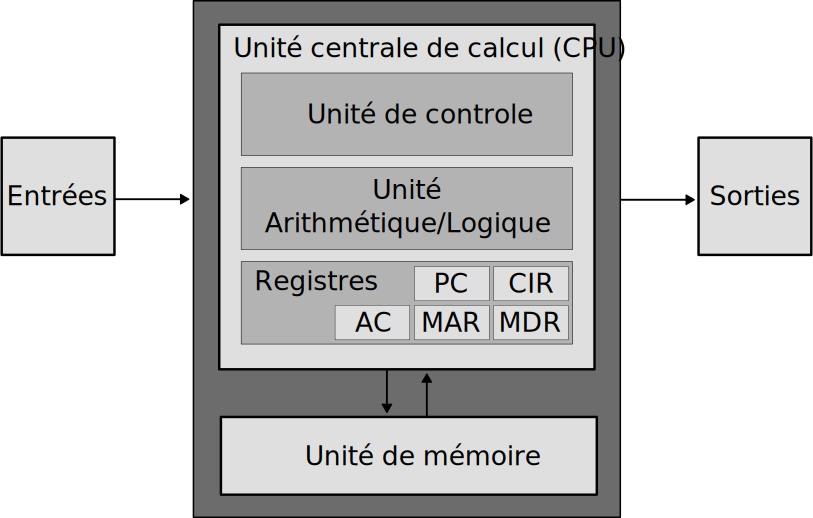
\includegraphics[width=.45\textwidth]{figures/Von-Neumann-Architecture-Diagram.jpg}
        \subcaption{Architecture de Von Neumann~\cite{tanenbaum2009modern}}
        \label{fig:sub1}
    \end{figure}
    \begin{block}{La mémoire idéale devrait être :}
        \begin{itemize}
            \item Extrêmement rapide
            \item Très grande
            \item Peu coûteuse
        \end{itemize}
    \end{block}

\end{frame}

\begin{frame}{Spoiler alert!}
    \begin{figure}
        \centering
        
\includegraphics[width=0.5\textwidth]{figures/meme.jpg}
        \label{fig:memory_speed}
    \end{figure}

    \begin{alertblock}{Problème}
        La technologie actuelle ne satisfait pas tous ces objectifs.
    \end{alertblock}
\end{frame}

\begin{frame}{Pourquoi ?}
    \begin{figure}[ht]
        \centering
        \centering
        \includegraphics[width=.75\linewidth]{figures/gap_cpu_ram_H.png}
        \subcaption{\'Ecart de performance entre CPU et
            RAMS~\cite{harris2021digital}}
        \label{fig:sub2}
    \end{figure}
    \begin{itemize}
        \item Les acc\`es mémoire sont nombreux et fréquents dans les
              programmes
        \item Les \'echanges de données entre la mémoire et le CPU sont lents.
              \begin{itemize}
                  \item Ordre de grandeur : $\times$ 100 plus lent pour accéder
                        à la RAM qu'aux registres
              \end{itemize}
        \item La performance des CPUs double tous les 18 mois (loi de Moore),
              celles des mémoires tous les $\simeq5$ ans
    \end{itemize}
\end{frame}

\begin{frame}
    \frametitle{Hiérarchie Mémoire}

    Questions :
    \begin{itemize}
        \item Quelles types de memoires connaissez-vous ?
        \item Quelle est le r\^ole de chacune de ces memoires ?
    \end{itemize}
\end{frame}

\begin{frame}
    \frametitle{Les différent types de mémoires}
    \begin{enumerate}
        \item \textbf{Registre} : Mémoire très rapide, très coûteuse et
              volatile. \\
              Contient les données de travail des unités de calculs.
        \item \textbf{Cache} : Mémoire rapide, coûteuse et volatile. \\
              Contient les données et instructions les plus utilisées par les
              unités de calculs.
              %   ($ \simeq 1-100 \$ / MB$)
        \item \textbf{Centrale} : Mémoire de vitesse moyenne, coût moyen et
              volatile. \\
              Contient les données et instructions des programmes en cours
              %   ($ \simeq 2-20 \$ / GB$)
        \item \textbf{Stockage} : Mémoire lente, peu coûteuse et non volatile
              (disques
              magnétiques/SSD). \\
              Contient les données et instructions des programmes non utilisés
              %   ($ \simeq 0.05-2 \$ / GB$)
    \end{enumerate}
    \begin{block}{Principe général}
        Plus une m\'emoire est rapide, plus elle est ch\`ere \`a
        fabriquer, plus sa taille est limit\'ee
    \end{block}

\end{frame}

\begin{frame}{Hiérarchie mémoire typique}
    \begin{figure}
        \centering
        \includegraphics[width=.75\textwidth]{figures/memory_speed_HH.png}
        \caption{Hiérarchie de la mémoire \cite{harris2021digital}}
    \end{figure}

    \begin{itemize}
        \item Le système de mémoire est construit comme une hiérarchie de
              couches.
        \item Chaque type de m\'emoire r\'epond \`a un objectif en terme de
              rapidit\'e/taille/co\^ut
    \end{itemize}
    \begin{block}{Principe de localité}
        Les programmes ont tendance à accéder aux mêmes données
        (\textbf{spatiale}) et instructions (\textbf{temporelle}) plusieurs
        fois.
        Il convient donc de garder les données fréquemment utilisées rapidement
        accessible pour le CPU.
    \end{block}
\end{frame}

\begin{frame}
    \frametitle{Registres}
    \begin{itemize}
        \item Premiere couche de la hiérarchie mémoire, integr\'es au CPU.
        \item Extrêmement rapides sans délai d'accès.
        \item Très faible capacité (moins de 1 KB).
        \item Deux types de registres : instructions et données.
        \item Utilisés pour stocker les données de travail des unites de
              calculs.
    \end{itemize}
    \begin{figure}
        \centering

        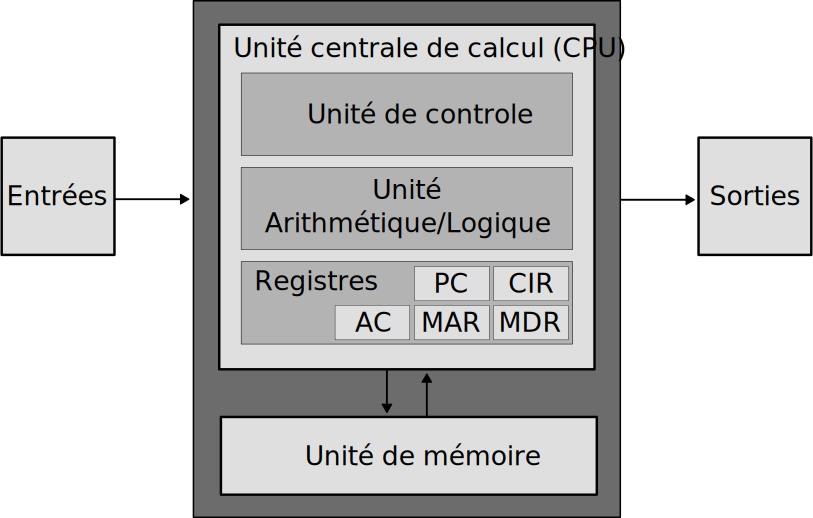
\includegraphics[width=.45\textwidth]{figures/Von-Neumann-Architecture-Diagram.jpg}
        \subcaption{Architecture de Von Neumann~\cite{tanenbaum2009modern}}
        \label{fig:sub1}
    \end{figure}

\end{frame}
\begin{frame}
    \frametitle{Mémoire Cache}
    \begin{itemize}
        \item Principalement contrôlée par le matériel
        \item Hiérarchique, avec plusieurs niveaux de cache
        \item Divisée en lignes de cache correspondant \`a la m\'emoire
              principale
        \item Taille limitée en raison de son coût élevé ($\simeq$
              1-100\$/MB)
    \end{itemize}
    \begin{block}{Composition d'une ligne de cache}
        \begin{itemize}
            \item \textbf{Données} : Contenu de la mémoire principale
            \item \textbf{Étiquette} : Adresse de la mémoire principale
            \item \textbf{Bits de contrôle} : Informations de contrôle
        \end{itemize}
    \end{block}
    \begin{figure}
        \centering
        \includegraphics[width=.5\textwidth]{figures/Direct_mapped_cache.JPG}
        \subcaption{Mémoire cache à correspondance préétablie (direct-mapped
            cache) [Wikipedia]}
    \end{figure}
\end{frame}

\begin{frame}
    \frametitle{Niveaux de Cache}
    \begin{itemize}
        \item \textbf{Redondance} : Les données stockées dans un niveau de
              cache
              sont également stockées dans les niveaux de cache supérieurs.
        \item \textbf{Hiérarchie} : Les niveaux de cache sont organisés en
              hiérarchie, du plus rapide et plus petit au plus lent et plus
              grand.
        \item \textbf{Localité} : Les données stockées dans un niveau de cache
              sont
              celles qui sont les plus susceptibles d'être utilisées par le
              CPU.
    \end{itemize}
    \begin{figure}
        \centering
        \includegraphics[width=.6\textwidth]{figures/ProcCoresCache_T.png}
        \subcaption{Mémoire cache~\cite{tanenbaum2009modern}}
    \end{figure}
\end{frame}

\begin{frame}
    \frametitle{Mémoire Principale}
    \begin{itemize}
        \item Basee sur la technologie DRAM (Mémoire à Accès Aléatoire
              Dynamique).
        \item Peut contenir des dizaines de gigaoctets dans les
              systèmes modernes.
        \item Toutes les demandes du CPU qui ne sont pas
              satisfaites par le cache vont à la mémoire principale.
        \item \textbf{Mémoire volatile} : les données sont perdues lorsque
              l'alimentation est coupée.
        \item Rafraîchissement périodique des données pour éviter la perte.
    \end{itemize}
\end{frame}

\begin{frame}
    \frametitle{Mémoire de Masse}
    \begin{block}{Principes}
        \begin{itemize}
            \item \textbf{Stockage non-volative} : les données sont conservées
                  même lorsque l'alimentation est coupée
            \item \textbf{Accès lent} aux données par rapport à la mémoire
                  principale0
            \item \textbf{Assurer la fiabilité} et la durabilité des données
                  stockées.
            \item \textbf{Stockage de grandes quantités de données} (plusieurs
                  TB)

        \end{itemize}
    \end{block}
    \begin{exampleblock}{Types de mémoire de masse}
        \begin{itemize}
            \item Disques durs (Hard Disk Drive)
            \item Disques à état solide (Solid State Drive)
            \item Disques optiques (CD-ROM)
            \item Bandes magnétiques (Grande capacité de plusieurs PB, faible
                  coût)
        \end{itemize}
    \end{exampleblock}
\end{frame}

\begin{frame}
    \frametitle{Mémoire Virtuelle}
    \begin{itemize}
        \item Permet d'exécuter des programmes plus grands que la mémoire
              physique.
        \item Utilise la mémoire principale comme cache pour les parties les
              plus exécutées.
        \item Gérée par l'UMM (Unité de Gestion de Mémoire).
        \item Supporte le multiprogrammation en gérant les commutations de
              contexte.
    \end{itemize}
\end{frame}

\begin{frame}
    \frametitle{Pas d'Abstraction de Mémoire}
    \begin{itemize}
        \item Modèles de mémoire sans abstraction.
        \item Exemples historiques : mainframes, minicomputers et premiers
              ordinateurs personnels.
    \end{itemize}
\end{frame}

\begin{frame}
    \frametitle{Les Souhaits des Programmeurs}
    \begin{itemize}
        \item Mémoire privée, infiniment grande et infiniment rapide.
        \item Mémoire non volatile et peu coûteuse.
        \item Réalité technologique actuelle : absence de telles mémoires.
    \end{itemize}
\end{frame}

\begin{frame}
    \frametitle{Modèles de Gestion de la Mémoire}
    \begin{itemize}
        \item Évolution des modèles de gestion de la mémoire.
        \item Gestion de la mémoire cache par le matériel.
        \item Modèle du programmeur de la mémoire principale.
    \end{itemize}
\end{frame}

\begin{frame}
    \frametitle{Gestion de la Mémoire}
    \begin{itemize}
        \item Importance de la mémoire principale (RAM) dans les systèmes
              informatiques.
        \item Croissance exponentielle des programmes par rapport à la mémoire
              disponible.
        \item Citation de la loi de Parkinson : « Les programmes s'étendent
              pour
              remplir la mémoire disponible. »
    \end{itemize}
\end{frame}

\begin{frame}
    \frametitle{Problèmes sans Abstraction de Mémoire}
    \begin{itemize}
        \item Conflits entre programmes écrivant sur les mêmes emplacements
              mémoire.
        \item Organisation de la mémoire avec le système d'exploitation et un
              seul
              processus utilisateur.
    \end{itemize}
\end{frame}

\begin{frame}
    \frametitle{Pagination}
\end{frame}

\begin{frame}
    \frametitle{Gestion des Espaces d'Adresses}
    \begin{itemize}
        \item Abstraction des espaces d'adresses par l'OS.
        \item Technique de pagination pour gérer les adresses.
    \end{itemize}

\end{frame}
\begin{frame}
    \frametitle{Exécution de Programmes Multiples sans Abstraction}
    \begin{itemize}
        \item Swapping : Sauvegarde de la mémoire sur un stockage non volatile.
        \item Exemple de l'IBM 360 avec des clés de protection pour la mémoire.
    \end{itemize}
\end{frame}

\begin{frame}
    \frametitle{Relocation Statique}
    \begin{itemize}
        \item Modification des programmes lors du chargement en mémoire.
        \item Ajout de constantes aux adresses de programme pour gérer la
              mémoire.
        \item Limites de la relocation statique.
    \end{itemize}
\end{frame}

\begin{frame}
    \frametitle{Mémoire Virtuelle}
    \begin{itemize}
        \item Concept de mémoire virtuelle pour gérer des espaces d'adresses
              plus
              grands que la mémoire physique.
        \item Rôle de l'OS dans la gestion des adresses et la mémoire physique.
    \end{itemize}
\end{frame}

\begin{frame}
    \frametitle{Mémoire Virtuelle}
    \begin{itemize}
        \item Notion de pages et cadres de pages
        \item Tables des pages
        \item Accélération de la pagination (TLB)
        \item Tables des pages pour les grandes mémoires
    \end{itemize}
    % \includegraphics[width=\textwidth]{virtual_memory_diagram.png}
\end{frame}

\begin{frame}
    \frametitle{Espaces d'Adresses}
    \begin{itemize}
        \item \textbf{Définition :} Un espace d'adresses est un ensemble
              d'adresses
              qu'un processus peut utiliser.
        \item \textbf{Concept de Base :}
              \begin{itemize}
                  \item Un ordinateur a de la mémoire principale (RAM) pour
                        exécuter les
                        programmes.
                  \item Dans un système d'exploitation simple, un seul
                        programme à la
                        fois peut être en mémoire (swapping).
              \end{itemize}
    \end{itemize}
    %\includegraphics[width=\textwidth]{simple_swapping_diagram.png}
\end{frame}

\begin{frame}
    \frametitle{Espaces d'Adresses dans les Systèmes d'Exploitation
        Sophistiqués}
    \begin{itemize}
        \item \textbf{Gestion de la Mémoire :}
              \begin{itemize}
                  \item Les systèmes sophistiqués permettent à plusieurs
                        programmes
                        d'être en mémoire simultanément.
                  \item Nécessité d'un mécanisme de protection pour éviter les
                        interférences.
              \end{itemize}
        \item \textbf{Rôle du Système d'Exploitation :}
              \begin{itemize}
                  \item Le système d'exploitation contrôle les mécanismes de
                        protection
                        fournis par le matériel.
              \end{itemize}
    \end{itemize}
    % \includegraphics[width=\textwidth]{multi_program_memory.png}
\end{frame}

\begin{frame}
    \frametitle{Mémoire Virtuelle et Gestion des Espaces d'Adresses}
    \begin{itemize}
        \item \textbf{Adresse Virtuelle vs Mémoire Physique :}
              \begin{itemize}
                  \item Adresses 32 bits (4 GB) ou 64 bits (16 EB) dépassent
                        souvent la
                        capacité de la mémoire physique.
                  \item La mémoire virtuelle permet de gérer plus d'espace
                        d'adresses que
                        la mémoire physique disponible.
              \end{itemize}
        \item \textbf{Fonctionnement :}
              \begin{itemize}
                  \item L'OS maintient une partie de l'espace d'adresses en
                        mémoire
                        principale et une autre partie sur SSD ou disque.
                  \item Les données sont échangées entre la mémoire principale
                        et le
                        stockage secondaire selon les besoins.
              \end{itemize}
    \end{itemize}
    % \includegraphics[width=\textwidth]{virtual_memory_diagram.png}
\end{frame}

\begin{frame}
    \frametitle{Problèmes de la Mémoire Physique Exposée}
    \begin{itemize}
        \item Risque de corruption du système d'exploitation par les programmes
              utilisateurs.
        \item Difficulté à exécuter plusieurs programmes simultanément.
        \item Besoin d'une abstraction pour protéger et gérer la mémoire.
    \end{itemize}
\end{frame}

\begin{frame}
    \frametitle{Notion d'un Espace d'Adresses}
    \begin{itemize}
        \item Définition d'un espace d'adresses : ensemble d'adresses qu'un
              processus peut utiliser.
        \item Chaque processus a son propre espace d'adresses, indépendant de
              ceux
              des autres processus.
        \item Exemple de numéros de téléphone, adresses IPv4 et domaines
              Internet.
    \end{itemize}
\end{frame}

\begin{frame}
    \frametitle{Introduction à la Mémoire Virtuelle}
    \begin{itemize}
        \item La mémoire virtuelle permet de gérer des programmes plus grands
              que
              la mémoire physique disponible.
        \item Importance dans les systèmes multi-tâches avec des programmes
              volumineux.
        \item Techniques historiques comme les overlays manuelles.
        \item Introduction du concept de mémoire virtuelle par Fotheringham
              (1961).
    \end{itemize}
\end{frame}

\begin{frame}
    \frametitle{Concept de la Mémoire Virtuelle}
    \begin{itemize}
        \item Chaque programme a son propre espace d'adressage, divisé en
              pages.
        \item Les pages sont mappées sur la mémoire physique mais pas toutes en
              même temps.
        \item Le matériel et le système d'exploitation gèrent le mapping et les
              pages manquantes.
    \end{itemize}
\end{frame}

\begin{frame}
    \frametitle{Pagination}
    \begin{itemize}
        \item Utilisation de la pagination pour la gestion de la mémoire
              virtuelle.
        \item Les adresses virtuelles sont traduites en adresses physiques par
              l'Unité de Gestion de Mémoire (MMU).
        \item Exemple d'un système de pagination avec des adresses de 16 bits
              et
              des pages de 4 KB.
    \end{itemize}
    % \includegraphics[width=\textwidth]{paging_example.png}
\end{frame}

\begin{frame}
    \frametitle{Tables de Pages}
    \begin{itemize}
        \item Les tables de pages mappent les pages virtuelles aux cadres de
              pages
              physiques.
        \item Chaque entrée de table de pages contient des informations comme
              le
              numéro de cadre de page et des bits de protection.
    \end{itemize}
    % \includegraphics[width=\textwidth]{page_table.png}
\end{frame}

\begin{frame}
    \frametitle{Entrée de Table de Pages}
    \begin{itemize}
        \item Exemple d'une entrée typique de table de pages : numéro de cadre
              de
              page, bit de présence/absence, bits de protection, etc.
    \end{itemize}
    % \includegraphics[width=\textwidth]{page_table_entry.png}
\end{frame}

\begin{frame}
    \frametitle{Accélération de la Pagination}
    \begin{itemize}
        \item Problème de performance avec les tables de pages en mémoire.
        \item Utilisation de TLB (Translation Lookaside Buffer) pour accélérer
              la
              traduction des adresses.
        \item Les TLB stockent les entrées fréquemment utilisées pour une
              traduction rapide.
    \end{itemize}
    % \includegraphics[width=\textwidth]{tlb.png}
\end{frame}

\begin{frame}
    \frametitle{Algorithmes de Remplacement de Pages}
    \begin{itemize}
        \item Algorithme de remplacement optimal
        \item Algorithme NRU (Not Recently Used)
        \item FIFO (First-In, First-Out)
        \item Algorithme Second-Chance
        \item Algorithme Clock
        \item LRU (Least Recently Used)
        \item Simulation de LRU en logiciel
        \item Algorithme de remplacement de pages de l'ensemble de travail
              (Working
              Set)
        \item Algorithme WSClock
    \end{itemize}
\end{frame}

\begin{frame}
    \frametitle{Gestion Logicielle des TLB}
    \begin{itemize}
        \item Sur certaines machines, la gestion des TLB est réalisée par le
              système d'exploitation.
        \item Différence entre les soft misses (pages en mémoire mais pas dans
              le
              TLB) et les hard misses (pages absentes de la mémoire).
    \end{itemize}
\end{frame}

\begin{frame}
    \frametitle{Tables de Pages pour Grandes Mémoires}
    \begin{itemize}
        \item Problème des grands espaces d'adressage virtuels.
        \item Utilisation de tables de pages multi-niveaux pour gérer de grands
              espaces d'adressage.
        \item Exemple de table de pages à deux niveaux.
    \end{itemize}
    % \includegraphics[width=\textwidth]{multilevel_page_table.png}
\end{frame}

\begin{frame}
    \frametitle{Exemple de Table de Pages à Deux Niveaux}
    \begin{itemize}
        \item Explication détaillée du fonctionnement de la table de pages à
              deux
              niveaux.
        \item Avantages de la réduction de l'utilisation de la mémoire.
    \end{itemize}
    % \includegraphics[width=\textwidth]{two_level_page_table.png}
\end{frame}

\begin{frame}
    \frametitle{Tables de Pages Inversées}
    \begin{itemize}
        \item Alternative aux tables de pages multi-niveaux : tables de pages
              inversées.
        \item Une entrée par cadre de page en mémoire réelle au lieu d'une
              entrée
              par page d'adresse virtuelle.
        \item Utilisation des TLB pour accélérer la traduction.
    \end{itemize}
    %\includegraphics[width=\textwidth]{inverted_page_table.png}
\end{frame}

\bibliographystyle{apalike}
\begin{frame}{Bibliographie}
    \bibliography{main}

\end{frame}
\end{document}
